\section{Representation}

The representer takes the results of the detection module and computes a \textit{representation} of each recognized object to be tracked. In the basic tracker, the representer extracts the BoundingBox and size of each blob and only keeps the biggest one as the single object being tracked.

The requirements in this module was to not only extract the bounding box and the size, but also determine the velocity and a local histogram for the object being tracked.

The velocity was calculated based on the location of the \textit{centroid} of the object being tracked as follows:

\begin{equation}
velocity = (centroid - old\_centroid) * fps
\end{equation}

where \textit{fps} is the frames per second in the video. Therefore, in this case we have to keep the centroid of the previous object being tracked.

For the histogram, we calculated the color histogram for the object being tracked.

\begin{figure}[Color histogram]{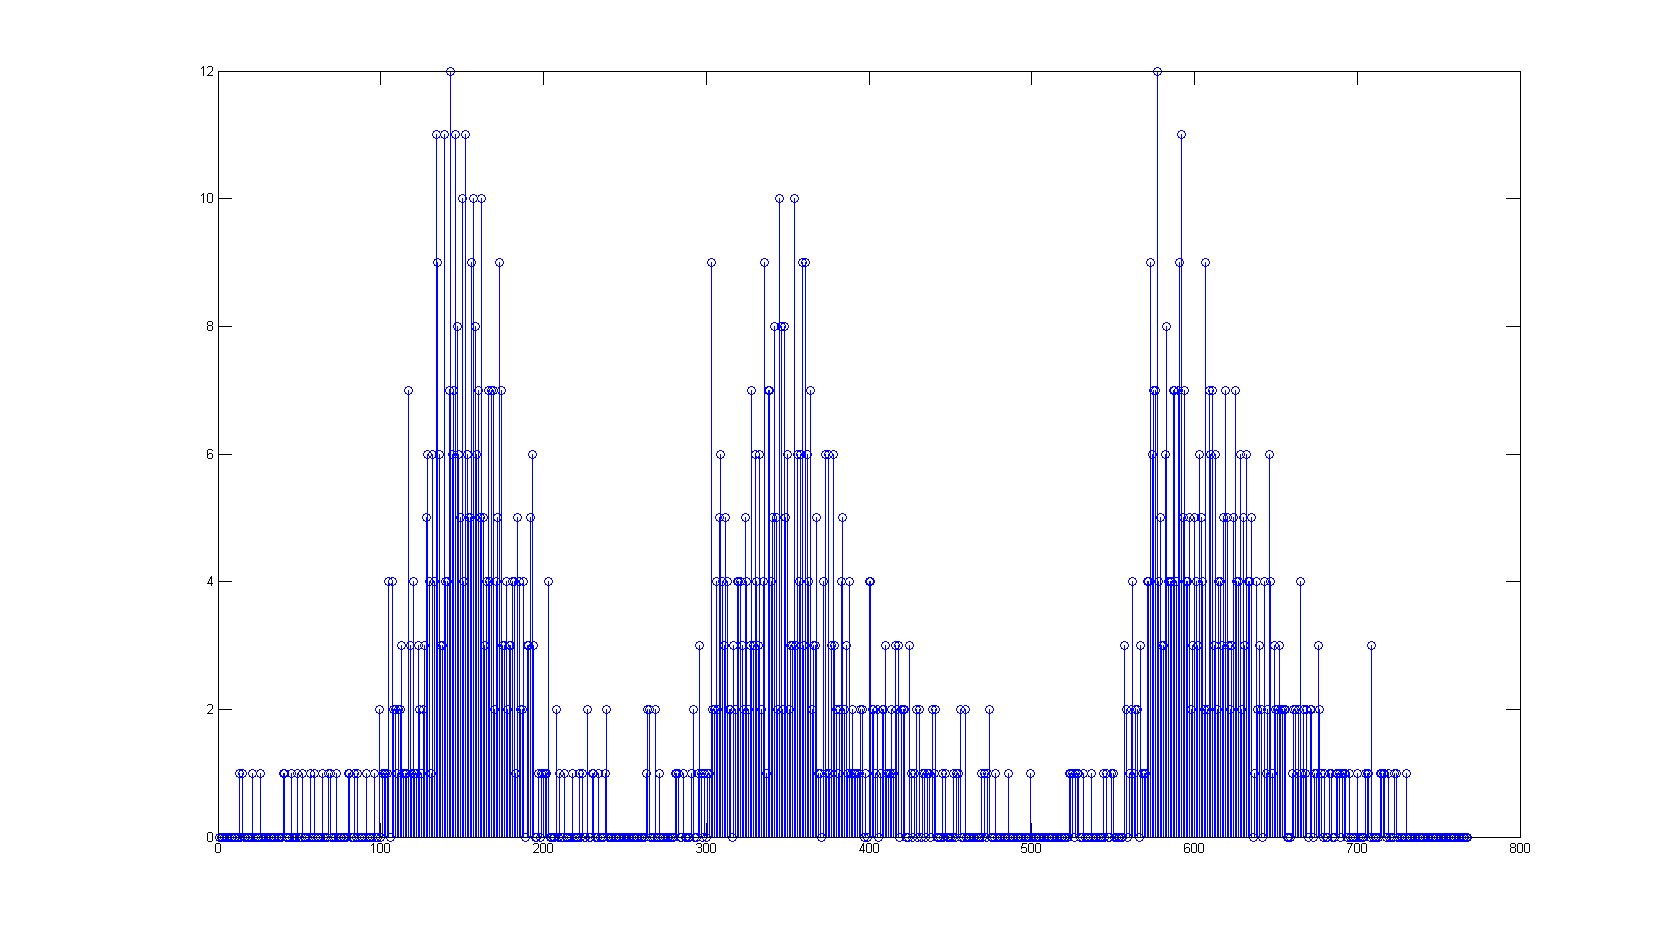
\includegraphics[width=0.9\textwidth]{histogram_car}}
  \centering
  \caption{RGB color histogram concatenated together on the same axis}
\end{figure}

According to our detection methodology. Our new representer now has to solve the correspondance problem between the detected objects in different frames. There are two cases that we have to consider.

Case 1, the detector already recognized the person. In this case we don't have to do anything. The correspondance probelm is already solved by the detector.

Case 2 is when the detector fails to detect the face of the person. However, this person is still in the scene. We then have to find a way to correspond the blobs in the scene with the people being tracked. We do this by getting the minimum euclidean distance between the previously represented blobs and the newely detected unrecognized blobs. We also make use of the prediction coming from the tracker as we try to find the minimum distance between the unrecognized blobs coming from the detector. In our case the usage of the color histogram will be redundant. The colors of the faces won't be of a high discriminative power for different blobs in the scene. However, If we have implemented the person's tracker. In this case it would had been an advantage to also make use of the colors histogram. Clothes of the people can be discriminative for the detected persons.
